\documentclass[11pt]{article}
\usepackage{theme}
\usepackage{shortcuts}
\usepackage{minted}
\usepackage[citestyle=alphabetic,bibstyle=alphabetic]{biblatex}
\addbibresource{main.bib}
\usemintedstyle{emacs}


\newenvironment{pseudocode}{
    \VerbatimEnvironment
    \begin{minted}[mathescape,
        %style=manny,
        linenos,
        numbersep=5pt,
        gobble=2,
        frame=lines,
        escapeinside=||,
        framesep=2mm,
        rulecolor=magenta]{python}%
}{
    \end{minted}%
}



% Document parameters
% Document title
\title{Mini-Project (ML for Time Series) - MVA 2023/2024}
\author{
Esteban Christiann \email{mailto:esteban.christiann@ens-paris-saclay.fr} \\ % student 1
Alexi Canesse \email{mailto:alexi.canesse@ens-lyon.fr} % student 2
}

\begin{document}
\maketitle

\paragraph{What is expected for these mini-projects?}
The goal of the exercise is to read (and understand) a research article, implement it (or find an implementation), test it on real data and comment on the results obtained.
Depending on the articles, the task will not always be the same: some articles are more theoretical or complex, others are in the direct line of the course, etc... It is therefore important to balance the exercise according to the article. For example, if you have reused an existing implementation, it is obvious that you will have to develop in a more detailed way the analysis of the results, the influence of the parameters etc... Do not hesitate to contact us by email if you wish to be guided.

\paragraph{The report}
 The report must be at most FIVE pages and use this template (excluding references). If needed, additional images and tables can be put in Appendix, but must be discussed in the main document. The report must contain a precise description of the work done, a description of the method, and the results of your tests. Please do not include source code! The report must clearly show the elements that you have done yourself and those that you have reused only, as well as the distribution of tasks within the team (see detailed plan below.)
 
 \paragraph{The source code}
In addition to this report, you will have to send us a Python notebook allowing to launch the code and to test it on data. For the data, you can find it on standard sites like Kaggle, or the site https://timeseriesclassification.com/ which contains a lot of signals!


\paragraph{The oral presentations}
They will last 10 minutes followed by 5 minutes of questions. The plan of the defense is the same as the one of the report: presentation of the work done, description of the method and analysis of the results.


\paragraph{Deadlines}
Two sessions will be available :
\begin{itemize}
 \item \textbf{Session 1}
 \begin{itemize}
  \item Deadline for report: December 18th (23:59)
  \item Oral presentations: December 20th and 22th (precise times TBA)
 \end{itemize}
\item \textbf{Session 2}
 \begin{itemize}
  \item Deadline for report: January 9th (23:59)
  \item Oral presentations: January, 11th and 12th (precise times TBA)
 \end{itemize}
\end{itemize}

\section{Introduction and contributions}

The Introduction section (indicative length : less than 1 page) should detail the scientific context of the article you chose, as well as the task that you want to solve (especially if you apply it on novel data). \textbf{The last paragraph of the introduction must contain the following information}:
\begin{itemize}
    \item Repartition of work between the two students\\
    
    Esteban : Inpainting, outlier detection and ringing removal.\\
    Alexi : Detrending, rereferencing, step removal.

    \item Use of available source code or not, percentage of the source code that has been reused, etc.\\
    
    The source code available is in matlab. This is a shitty language and releasing a paper with only a matlab implementation is equalivalent to not releasing source code. Furthermore, it was poorly written and unreadable without any damn documentation. We only looked at the code to get the details missing in the paper because the paper lacks details. (freaking learn to write dammit). AND FOR GOD'S SAKE \(d(t) \neq d\). Writting things like \(d(t)/std(d(t))\) makes you look like a five years old.

    \item Use of existing experiments or new experiments (e.g. test of the influence of parameter that was not conducted in the original article, application of the method on a novel task/data set etc.)\\
    
    TODO
    \item Improvement on the original method (e.g. new pre/post processing steps, grid search for optimal parameters etc.)\\
    
    TODO
\end{itemize}

\section{Method}

The following section presents the algorithms proposed by the paper and gives pseudo-code for each algorithm.

\subsection{Robust detrending}

The main issue with usual detrending methods is that they are sensible to artefacts that are common in EEG and MEG data. They therefore present an algorithm that takes this into account. We fit a trend to the data and where the residuals are over a threshold, we flag the point as an outlier and do not take it into account to fit a the basis anymore. This is iterated a few times and gives great results. 

\begin{pseudocode}
detrending(signal):
    weights = [1, 1, |\(\dots\)|, 1] # weights for outlier detection (0 means outlier)
    iterrate |\(n_\text{iter}\)| times:
        projected_signal = fit_to_basis_using_weights(signal, weights)
        error_on_projection = abs(signal - projected_signal)
        for t in len(signal):
            if error_on_projection[t]/std(error_on_projection) > threshold:
                weights[t] = 0
            else:
                weights[t] = 1
    return signal - fitted_signal # detrended signal
\end{pseudocode}

\subsection{Inpainting}

Motion of the electrodes or leads can create temporally-localized glitches. Given the list of glitches for each channel, one could try to reconstruct the signal at these timesteps to remove these glitches. This process is called \emph{inpainting}. Using a signal model where there is linear redundancy accross channels, the authors formulate an inpainting algorithm that first estimate the linear relationship between channels and use it to reconstruct the signal on timesteps affected by glitches.


\begin{pseudocode}
inpaint(x, w):
    N = Number of channels
    for n in range(N):
        Partition the time axis into |\(K\)| subsets based on validity of channels
        for k in range(K):
            T_k = timesteps in subset k
            Tprime = subset of T_k where ch. n is valid
            Tinpaint = subset of T_k where ch. n has to be reconstructed
            Estimate the linear relationship between ch. n and valid ch. on Tprime
            Use the relationship to reconstruct ch. n on Tinpaint
    return new_x
\end{pseudocode}

\subsection{Outlier detection}

The inpainting algorithm need the locations of glitches. This is what the outlier detection algorihm computes. It uses the inpainting algorithm multiple times and flag as outliers the poorly reconstructed values for the next iteration.

\begin{pseudocode}
outlier_detection(x, thres=2., maxiter=20):
    w = ones_like(x) # Initially assume there are no outliers
    for it in range(maxiter):
        xbar = inpaint(x, w) # Try to reconstruct the data
        d = np.abs(x - xbar)
        w = d < thres * d.std() # Flag high reconstruction errors as outliers
    return w
\end{pseudocode}

\subsection{Robust rereferencing}

Rereferencing is subtracting the average over all channels to the data. It is used because EEG measures are potentials therefore relative. When applying rereferencing, one corrupted channel can then affect every channels. To prevent this, the mean computed is computed only on values that are not outliers according to the outlier detection algorithm. Another solution is to use the output of the inpainting algorithm instead of the raw data.

\begin{pseudocode}
rereferencing(signal):
    weights = 1 - outlier_detection(signal) # 1 : valid data / 0 : outlier
    weighted_mean = mean_using_weights(signal, weights)
    return signal - weighted_mean
\end{pseudocode}

\subsection{Step removal}

The algorithm has two parts, first, it detects steps and then it removes them. In order to detect steps, the algorithm look at the empirical variance from the beginning and from the end and recursively look for the next step until it can't find any or the max depth is reached. We suspect that this part of the algorithm could be improved using change point detection methods we have seen in the fifth lab. However, we did not compared them because the proposed solution already worked more than well enough.

\begin{pseudocode}
# Recursively look for steps in the signal
step_detection(signal, depth)
    |\(\forall (t,T)\)| M[t][T] = mean(x[t:T+1])
    |\(\forall (t,T)\)| V[t][T] = |\(\sum_{i=t}^T (x_i - M_t^T)^2\)|
    
    t0 = argmin(V[1][t] + V[t][T], t) # most likely position to be a step
    if not(is_step(signal, t0)): # Check if t0 is indeed the position of a step
        return [] # no steps
    
    # Check for steps on both sides of t0
    steps_left = step_detection(signal[:t0], depth - 1)
    steps_right = t0 + step_detection(signal[t0:], depth - 1) # + t0 because signal si shifted

    return concatenate(steps_left, [t0], steps_right)

step_removal(signal, depth):
    steps = step_detection(signal, depth)

    for step in steps:
        signal[steps:] -= difference_mean_before_and_after_step(signal, step)

    return signal # Without steps

\end{pseudocode}

\subsection{Ringing removal}

Ringing artefacts are caused by the antialiasing filter at the MEG steps. The authors suggest to use a small portion of the signal after each step to estimate the effect of the antialiasing filter and cancel it, which removes ringing artefacts.

\begin{pseudocode}
ringing_removal(x, step_list):
    for n in range(number of channels):
        for step in step_list[n]:
            Estimate filter parameters on x[step : step + 100, n]
            imp_res = impulse response of the filter
            x[step : step+100, n] -= imp_res
\end{pseudocode}


\section{Data}
MEG and EEG data are medical recordings which make them a scare ressource. They should also be shared with great care. We used data from~\cite{Litvak2016}, the same data as the one used in the original article. The protocol used to record these MEG signals are described in ~\cite{oswal2016analysis}. The recordings we used are from ``phantom090715\_BrainampDBS\_20150709\_07.ds'' because this dataset is described as being the most realistic.\\

The data is sampled at 2,400Hz. Each recording is 4 minutes long and contains 303 channels. The data contains artefacts such trends, steps, ringing and outliers that are inherent to MEG recordings. Those have been presented in introduction.\\

We did not pre-process our data as the algorithms we use are the main steps of pre-processing. Only denoising is not presented in the methods here. We did not applied any denoising because denoising should be applied \textit{after} the application of the methods presented in the article. Indeed, artefacts could greatly impact denoising. Furthermore, MEG data is complicated and we do not understand the field enough to even know when we would remove actual data. The authors of the recording implemented two sensor-level denoising methods. They first used S3P-a technique based on eigenvalue decomposition of the complex cross-spectral density matrix (this technique is similar to SSA studied in the lectures); the second is pTSSS which defines subspaces using singular value decomposition. These successfully removed artefacts related to the stimulation and low level frequencies. However, this did not improved their ability to perform the task of their experiment.\\

We also manually generated some signals using the sum of a polynomial and white noise on top of which we added an artificial glitch. This was meant to be easy to use and interpret data.\\ 

\section{Results}
The Result section (indicative length : 1 to 2 pages) should display numerical simulations on real data. If you re-used some existing implementations, it is expected that this section develops new experiments that were not present in the original article. Results should be discussed not only based on quantitative scores but also on qualitative aspects. In particular (especially if your article focuses on black box methods), please provide some feedbacks whether the method was adapted to the data or not and whether the hypothesis behind the approach you used were validated or not.

We applied the following preprocessing pipeline to a subset of 16 channels of the raw MEG data.

\begin{figure}
    \centering
    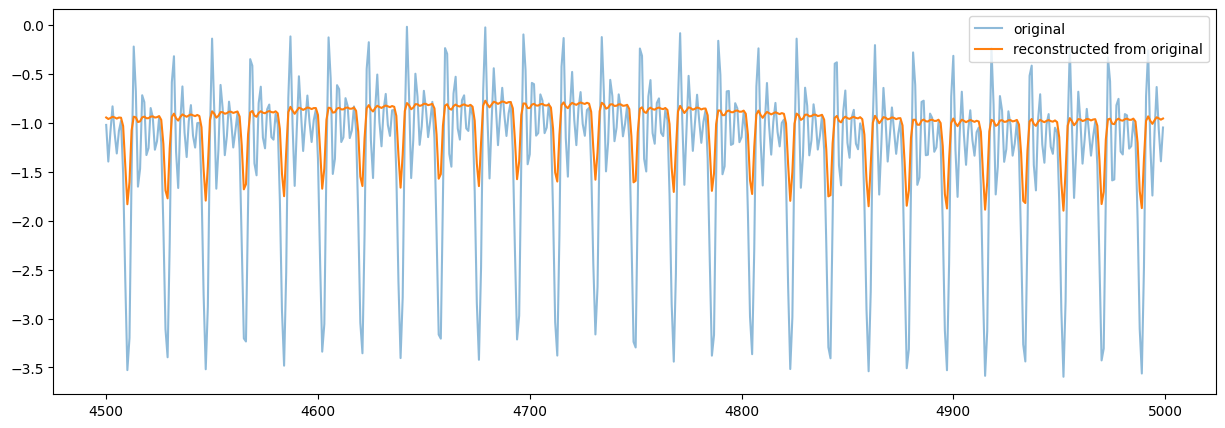
\includegraphics[width=12cm]{recons.png}\\
    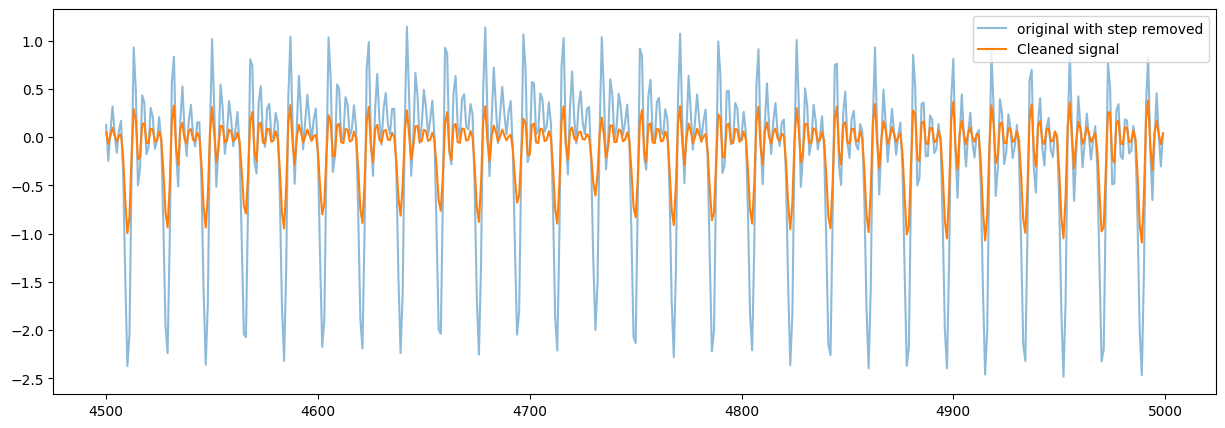
\includegraphics[width=12cm]{recons_clean.png}
    \caption{Top: Raw MEG and its reconstruction. Bottom: Cleaned MEG with its reconstruction}
\end{figure}

\newpage

\printbibliography[heading=bibintoc]


\end{document}
